\section{Evaluation}

We used two complementary studies to separate the effect of exposing editable semantic decisions (RQ2--RQ3) from the effect of conversational context on the proposed interpretation itself (RQ1). Study~A compares end-to-end authoring workflows in Maya; Study~B compares text-only Dialogue-Only and Full-Context proposals (Figure~\ref{fig:study-design}).

\begin{figure*}[t]
    \centering
    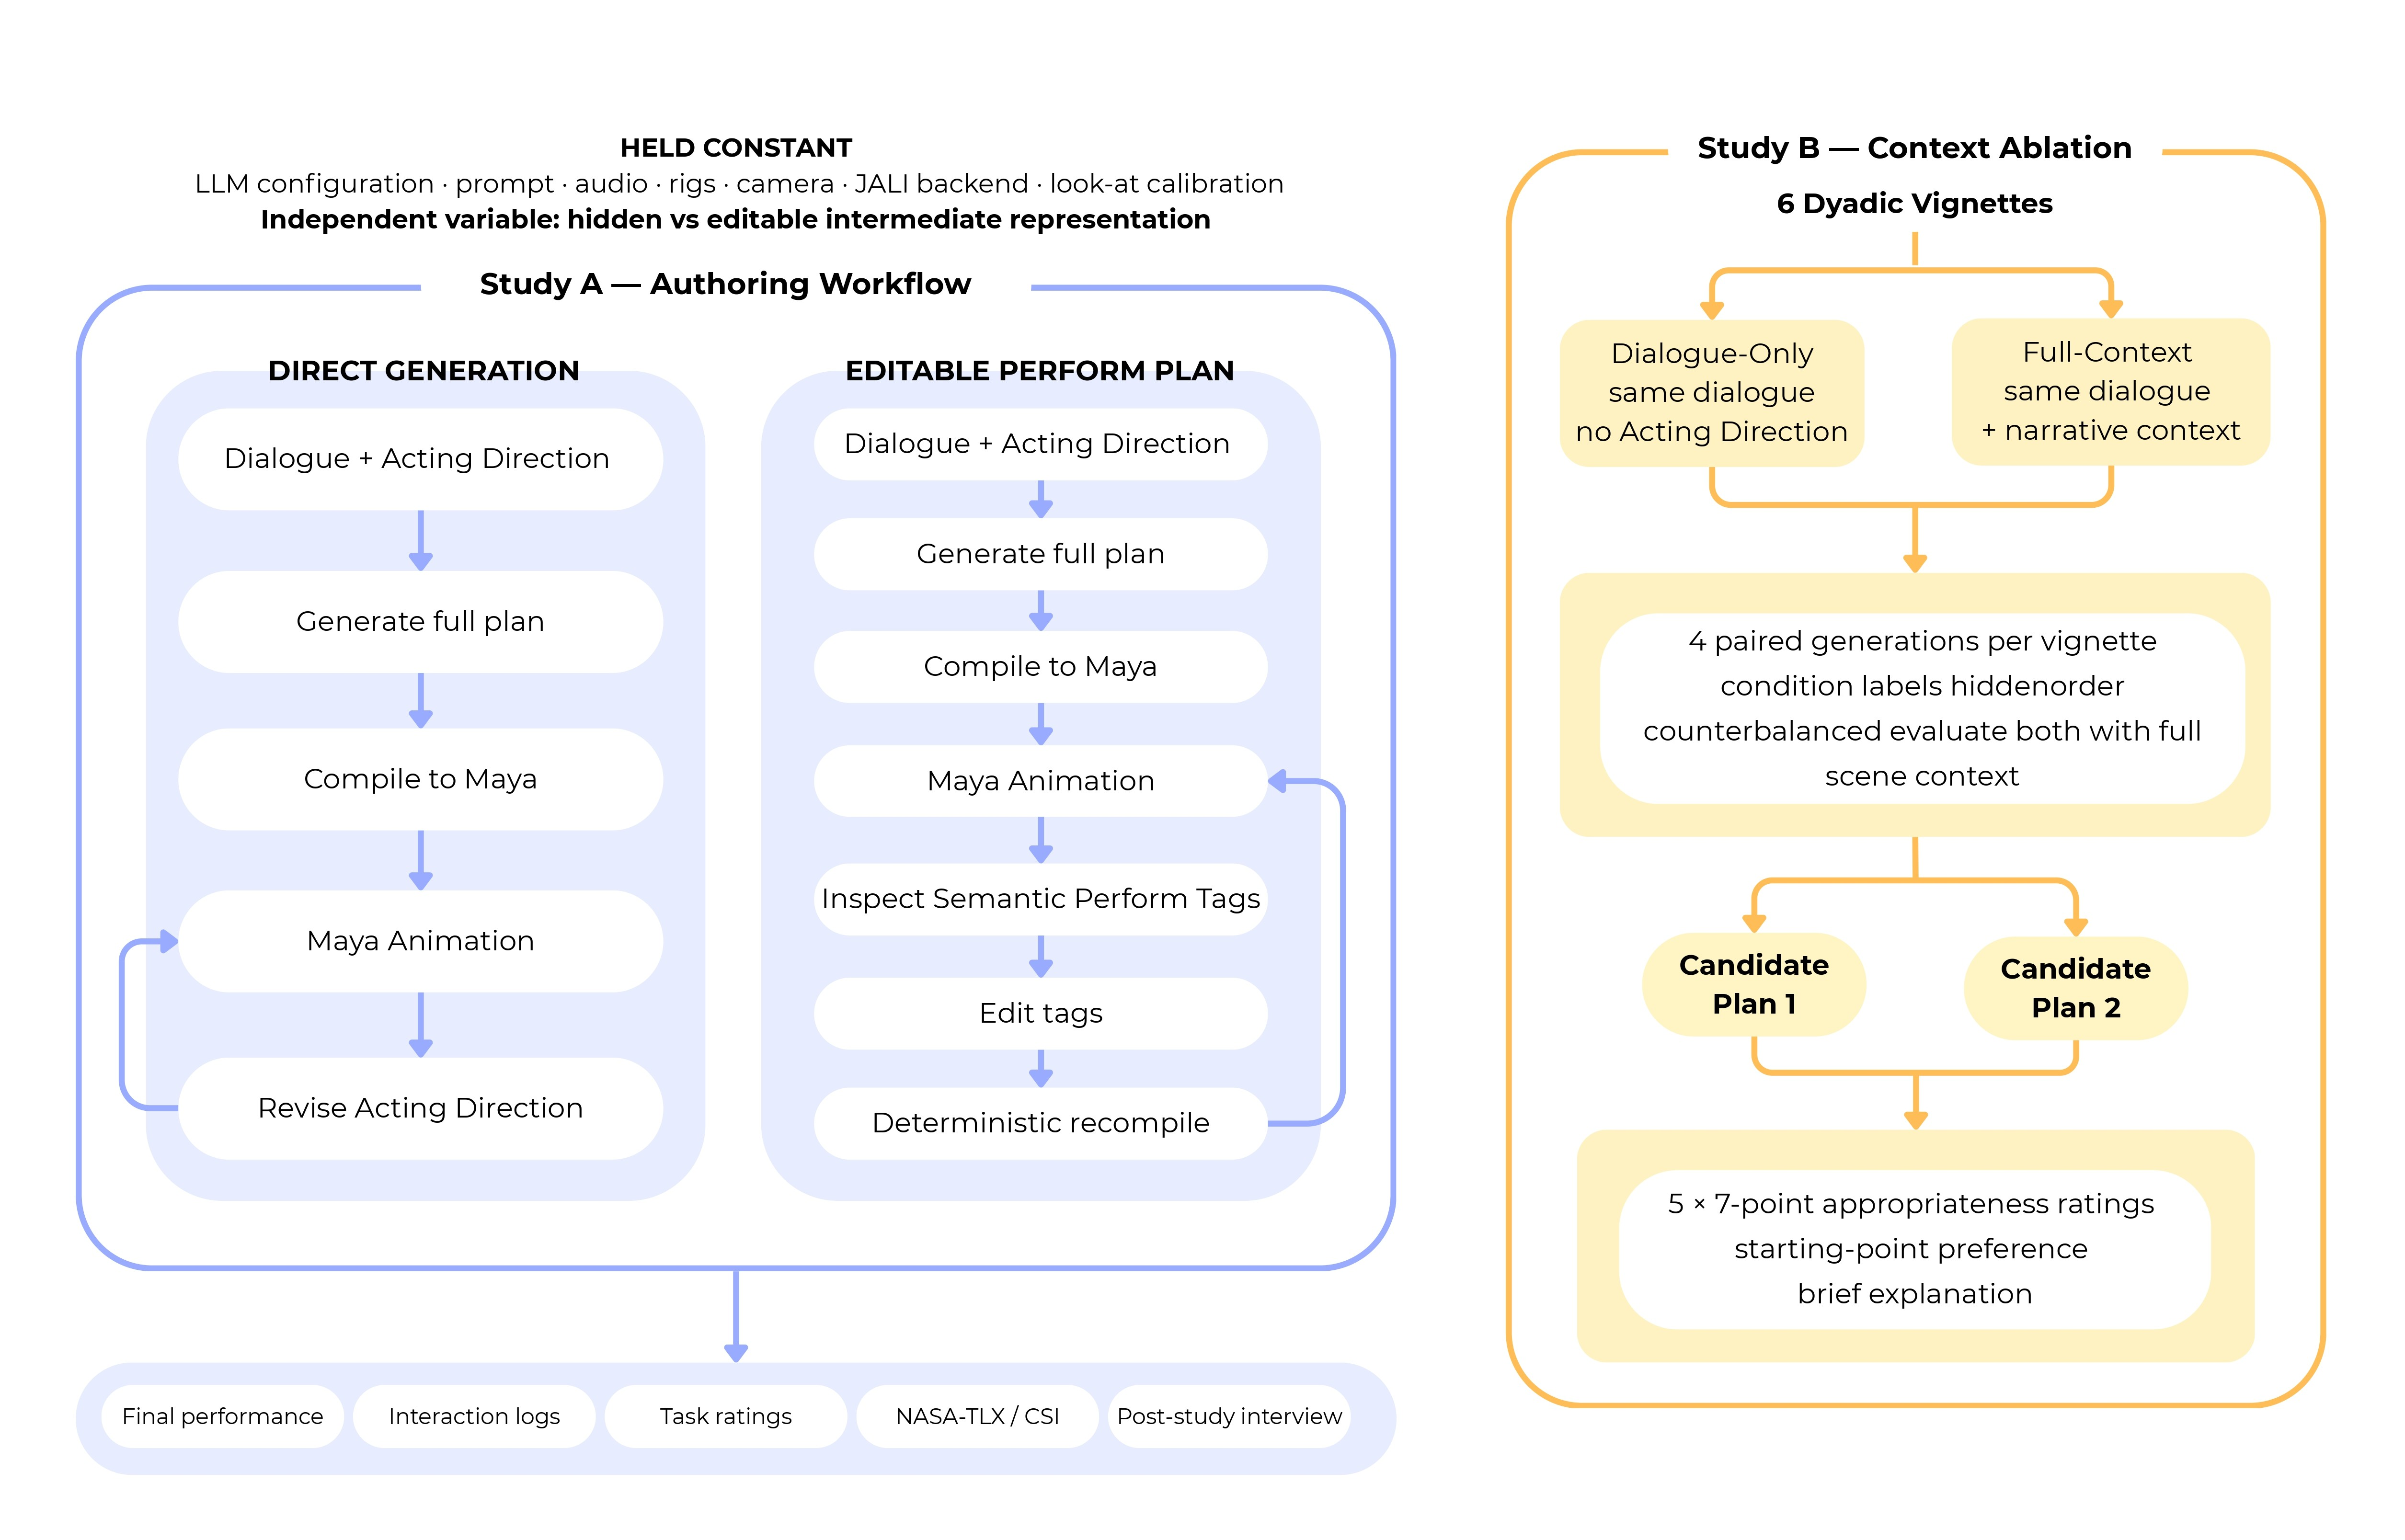
\includegraphics[width=\textwidth]{figures/evaluation_design.jpg}
    \caption{Two-part evaluation. Study~A compares Direct Generation with Editable Semantic Performance Tags in Maya while holding the generation and execution stack constant. Study~B isolates the effect of contextual information on text-only performance proposals across six dyadic vignettes.}
    \Description{Study A is a within-subject comparison between Direct Generation and Editable Semantic Performance Tags. Study B compares Dialogue-Only and Full-Context proposals across six vignettes with condition labels hidden and presentation order counterbalanced.}
    \label{fig:study-design}
\end{figure*}

\subsection{Participants and Overall Procedure}

We analyzed 16 usable participant records. Participants had character-animation or related performance-authoring backgrounds spanning game/film animation, animation/VFX study, professional character animation, and technical animation. Because roles could be selected jointly, eight participants reported game/film animation backgrounds, seven animation/VFX study, three professional animation, and one technical-animation/TD experience. Thirteen reported a numeric duration of relevant experience, spanning 2--15 years ($M=4.69$, $SD=3.54$). Of the 15 participants who completed at least one software-background item, all reported Maya or another keyframe-animation package.

Participants received an explanation of the Semantic Performance Tag fields and completed a short practice example before the formal tasks. The same participants then completed the end-to-end authoring tasks and the text-only context-ablation ratings. Formal stimuli used in Study~A and Study~B did not overlap, and the Study~A tutorial scene was excluded from analysis.

\subsection{Study A: Authoring Workflow Comparison}

\subsubsection{Tasks and Conditions}

Study~A examined whether editable Semantic Performance Tags changed how participants revised system-generated conversational performances. After one tutorial, participants authored both interlocutors in four short dyadic scenes chosen to span complementary context-dependent acting problems such as concealment or suspicion, restrained or affectively incongruent response, evolving interpersonal tension, and relationship repair. Scenes contained exactly two speaking characters and were kept short and comparable in scope. The goal was to make each result match the participant's own reading rather than a reference performance.

The implementation used the same generation and execution path in both conditions; only the visibility and editability of the intermediate semantic representation differed. Both conditions used the same model configuration, dialogue, Acting Direction, scene audio, rigs, cameras, JALI backend, and pre-calibrated semantic look-at targets. Direct low-level Maya curve editing was excluded so that the comparison primarily reflected prompt-level regeneration versus semantic-tag editing.

\paragraph{Direct Generation.}
Participants viewed the generated JALI/Maya animation with the intermediate semantic representation hidden. To revise the acting, they changed the natural-language Acting Direction and regenerated the complete proposal and animation.

\paragraph{Editable Semantic Performance Tags.}
Participants received the same initial dialogue, Acting Direction, model configuration, and generated animation, but could additionally inspect two character-specific tag panels. They could edit affect, persistent or temporary attention, head, and performative-blink decisions across either character. Valid edits updated the existing canonical plan and were deterministically recompiled without another LLM call. The current prototype does not provide field locking or selective LLM regeneration.

Each participant completed two Direct Generation scenes followed by two Editable Semantic Performance Tag scenes. Because workflow order was fixed in the collected sessions, we treat Study~A as a paired first-use comparison and interpret differences with a possible practice/order effect rather than as order-independent causal estimates.

\subsubsection{Interaction Records and Measures}

The prototype retains the original generated canonical plan, edited canonical-plan snapshots where saved, and sidecar session records. These can expose semantic value changes and retained decisions by character and channel (affect, gaze/attention, head, and blink). However, early sessions were not instrumented uniformly enough to support a complete action-by-action reconstruction across all participants. We therefore do not infer population-level accept/modify/remove rates from missing logs; RQ3 is discussed only where saved plan differences directly support the observation.

After each authoring task, participants rated match to intended reading and final satisfaction on seven-point scales. After each two-task workflow block they completed the six raw NASA-TLX dimensions \cite{hart1988nasa} and nine study-specific seven-point workflow items covering expression of acting direction, local revision, revision clarity, final control, dyadic coordination, visual--semantic iteration, creative ownership, alternative exploration, and whether quality justified effort. Items are reported individually rather than as an unvalidated composite. After the editable-tag block, three diagnostic ratings assessed tag-level fit, usefulness of phrase-level interpretation, and the dual-character layout; these were not included in between-workflow tests.

The semi-structured post-study interview focused on the process behind observed edits rather than endorsement of predefined features. It asked how participants judged a performance as complete, what system-proposed decisions they kept, changed, or removed, what they changed first after a mismatch, how prompt regeneration compared with tag editing for alternatives and preservation, where facial channels interacted, whether the dual-character layout aided coordination, when phrase-level interpretations were useful, how semantic gaze targets related to camera/rig decisions, whether the workflow affected authorship or control, and what operations or semantic fields were missing.

\subsubsection{Study A Analysis}

For the two task-level outcomes, we averaged each participant's two tasks within workflow and required two valid task ratings in each workflow. One participant had ambiguous double selections on one Editable-tag task, so the paired task-level tests use $n=15$. The nine workflow items were analyzed item-wise using all valid paired responses ($n=13$--16), and all six NASA-TLX dimensions had $n=16$ paired responses. Given the small sample and ordinal questionnaire outcomes, we use two-sided Wilcoxon signed-rank tests, rank-biserial correlations, and Holm correction within the task-outcome, workflow-item, and NASA-TLX families. Positive rank-biserial values indicate higher Editable-tag ratings; for NASA-TLX, higher values indicate greater workload except performance, where 0 denotes perfect performance and 100 failure.

\subsection{Study B: Context Ablation}

\subsubsection{Stimuli and Conditions}

Study~B isolates semantic interpretation from animation execution and tests whether additional narrative and interpersonal context changes the appropriateness of the proposed performance itself. We constructed six short dyadic vignettes using maximum-variation sampling across contextual dependence and interactional function. Two relatively explicit supportive or confrontational vignettes served as lower-context-dependence cases; four higher-context cases involved concealment, face-saving, tentative affiliation, and relationship repair (Table~\ref{tab:study-b-stimuli}). The vignettes contained no prescriptive facial-animation directions such as named expressions, gaze instructions, head gestures, or blink commands. Context descriptions specified only narrative facts, character relationships, and relevant prior events, leaving performance interpretation to the model.

\begin{table}[t]
    \centering
    \caption{Study~B stimuli vary contextual dependence and interactional function.}
    \label{tab:study-b-stimuli}
    \begin{tabular}{lll}
        \toprule
        \textbf{ID} & \textbf{Context dependence} & \textbf{Interactional problem} \\
        \midrule
        S1 & Low & Explicit support \\
        S2 & Low--moderate & Explicit conflict \\
        S3 & High & Concealment \\
        S4 & High & Face-saving / mixed affect \\
        S5 & High & Tentative affiliation \\
        S6 & High & Relationship repair \\
        \bottomrule
    \end{tabular}
\end{table}

For each vignette we generated shared dyadic proposals under two conditions while holding the model, prompt schema, identities, and decoding configuration constant. Dialogue-Only received labeled dialogue and character identities; Full-Context received the same dialogue plus narrative and interpersonal context through Acting Direction. We generated four independent Dialogue-Only/Full-Context pairs for each vignette, yielding 48 proposals. The replicate pairs were distributed across 16 preconstructed participant packets so that each pair appeared equally often and Dialogue-Only versus Full-Context appeared first equally often across assignments.

The ablation applied only to model input: raters always saw the complete vignette context and dialogue. Each trial showed two anonymized text-only proposals as Plan~A and Plan~B, with hidden condition labels and counterbalanced order; no animation was shown.

\subsubsection{Measures and Analysis}

For each anonymous proposal, participants rated five seven-point criteria (1 = not at all appropriate; 7 = extremely appropriate): overall contextual appropriateness, acting intention, affect, attention/gaze, and dyadic coordination/temporal placement. They then selected Plan~A, Plan~B, or No preference as the preferred animation starting point and could briefly explain the choice.

For each criterion, we averaged the six Dialogue-Only and six Full-Context ratings within participant and compared paired participant-level values with two-sided Wilcoxon signed-rank tests. Overall fit, intention, affect, and gaze use all 16 complete participant pairs; timing uses 15 because one Full-Context timing rating was missing. We report rank-biserial correlations and Holm-adjusted $p$ values across the five criteria. Starting-plan choices are decoded back to condition and reported descriptively across all 96 scene-level questions, retaining No preference, missing, and ambiguous responses separately. Open-ended responses are used only as qualitative context; we make no thematic-frequency claims from questionnaire comments alone.
